\documentclass[xetex,mathserif,serif]{beamer}
\usepackage{polyglossia}
\usepackage{minted}
\usepackage{tabu}

\usepackage{textpos}
\setlength{\TPHorizModule}{1cm}
\setlength{\TPVertModule}{1cm}

\useoutertheme{infolines}

\usepackage{fontspec}
\setmainfont{FreeSans}
\newfontfamily{\russianfonttt}{FreeSans}

\setbeamertemplate{blocks}[rounded][shadow=false]
\setbeamercolor*{block title example}{fg=green!50!black,bg=green!20}
\setbeamercolor*{block body example}{fg=black,bg=green!10}

\setbeamercolor*{block title alerted}{fg=red!50!black,bg=red!20}
\setbeamercolor*{block body alerted}{fg=black,bg=red!10}

\definecolor{cadmiumgreen}{rgb}{0.0, 0.42, 0.24}

\tabulinesep=0.7mm

\title{REAL.NET}
\author[Юрий Литвинов]{Юрий Литвинов \newline 
	\textcolor{gray}{\small\texttt{y.litvinov@spbu.ru}}
}

\date{28.09.2017}

\begin{document}

	\begin{frame}
		\frametitle{REAL.NET}
		\begin{columns}
			\begin{column}{0.5\textwidth}
				\begin{itemize}
					\item Среда для быстрого создания визуальных языков
					\item Зачем:
					\begin{itemize}
						\item End-user programming
						\item Обучение
						\item Научные эксперименты
						\item ...
					\end{itemize}
					\item Ближайшие цели:
					\begin{itemize}
						\item Программирование роботов
						\item ``Умная теплица''
						\item Программирование квадрокоптеров
					\end{itemize}
				\end{itemize}
			\end{column}
			\begin{column}{0.5\textwidth}
				\center{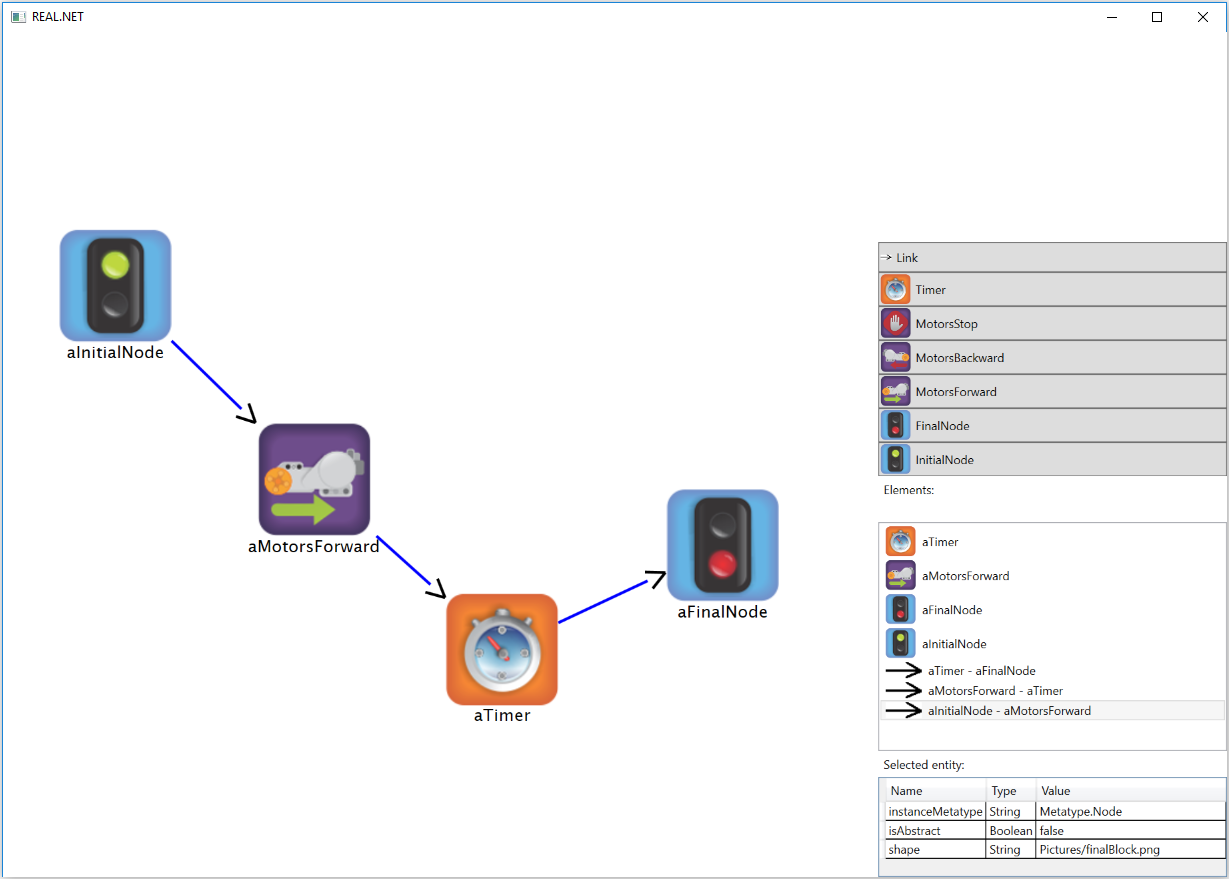
\includegraphics[width=0.9\textwidth]{realNet.png}}
			\end{column}
		\end{columns}
	\end{frame}

	\begin{frame}
		\frametitle{Техническая часть}
		\begin{itemize}
			\item Наука: предметно-ориентированные графические языки, метамоделирование
			\item Технологии: .NET (C\#, F\#), WPF, WinForms
			\item Ссылка на репозиторий: \url{https://github.com/yurii-litvinov/REAL.NET}
			\item Контакты: \texttt{yurii.litvinov@gmail.com}
			\item Предыдущие результаты: QReal, TRIK Studio
		\end{itemize}
		\center{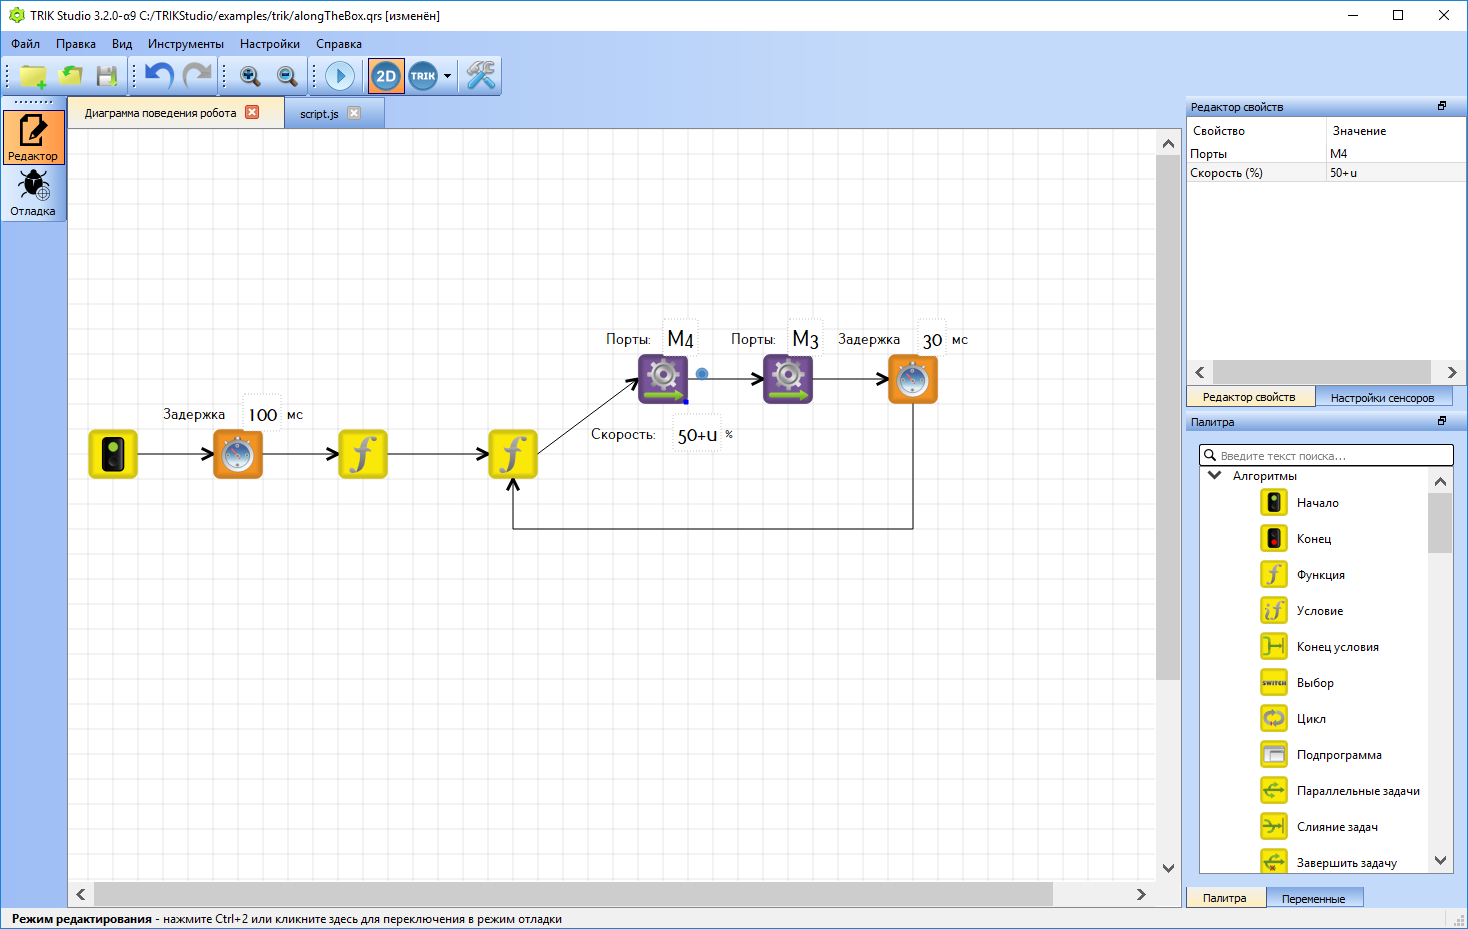
\includegraphics[width=0.4\textwidth]{trikStudio.png}}
	\end{frame}

	\begin{frame}
		\frametitle{Задачи}
		\begin{itemize}
			\item Продвинутый редактор графов
			\begin{itemize}
				\item Плагинная система
				\item Сетка, выравнивание элементов
				\item Поддержка портов на узлах
				\item Аккуратное рисование связей
				\item Редактирование свойств
				\item Переключение между моделями
				\item Редактирование языка ``на лету''
			\end{itemize}
			\item Продвинутый репозиторий
			\begin{itemize}
				\item Сохранение/загрузка
				\item Импорт/экспорт из популярных форматов
			\end{itemize}
			\item Общеархитектурные вопросы
			\begin{itemize}
				\item Заменяемые редакторы
				\item Модуляризация и переиспользование из .NET-приложений
			\end{itemize}
		\end{itemize}
	\end{frame}

\end{document}

